\documentclass{report}  
\usepackage[utopia]{mathdesign} 
%\usepackage{amsmath,amsfonts,amsthm,amssymb,mathtools}

\input{preamble.tex}

\usepackage{amsmath,amsthm,mathtools}



%\usepackage[scr]{rsfso}

%\usepackage{libertine}
%\usepackage{mathpazo}
%\usepackage{palatino}
%usepackage{crimson}


\newcommand{\faketarget}{\oplus\!\!\!\!\odot}
\newcommand{\target}{%
  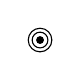
\begin{tikzpicture}[scale=0.5]
    \fill[black] (0,0) circle (0.1);
    \draw (0,0) circle (0.2);
    \draw (0,0) circle (0.3);
  \end{tikzpicture}%
}

\usepackage[clock]{ifsym}


\title{\Huge{Interface Personne Marchine}\\{IFT2905}\\{\textbf{Introduction}}}
\author{\huge{Franz Girardin}}
\date{\today}
\lstset{inputencoding=utf8/latin1}

            %%%%%%%%%%%%%%%%%  Sect.                          %%%%%%%%%%%%%%%%%%%%%%%%%%%%%%%%%%%%%%%%%%%%%%%%%%%%%%%%%
\usepackage{helvet}
\titleformat{\chapter}
  {\fontfamily{phv}\bfseries\huge} % format
  {}                % label
  {0pt}             % sep
  {\color{myb}\huge}           % before-code



\titleformat{\section}
  {\normalfont\scshape}{\thesection}{1em}{}


% Customizing the spacing for the chapter titles
\titlespacing*{\chapter}{0pt}{0pt}{20pt}

%\usepackage[utopia]{mathdesign}
% Allow hfill in math environment
\newcommand{\specialcell}[1]{\ifmeasuring@#1\else\omit$\displaystyle#1$\ignorespaces\fi}

% Allow you to do the non implication (implication barred)
\newcommand{\notimplies}{%
  \mathrel{{\ooalign{\hidewidth$\not\phantom{=}$\hidewidth\cr$\implies$}}}}



\DeclareRobustCommand{\looongrightarrow}{%
  \DOTSB\relbar\joinrel\relbar\joinrel\relbar\joinrel\rightarrow
}

\begin{document}
%\maketitle

\pagebreak

\pagebreak
\begin{multicols*}{3}


    \footnotesize
    %\section*{Design of everyday things}


    \paragraph{Mythe de l'erreur humaine} $\mathcal{H}$   
    Les \textit{échecs} d'un système $\mathbb{PM}$ sont souvent dus  
    au \textbf{design}. Pour $\downarrow$ erreur $\mathcal{H}$ : 
    \begin{itemize}
        \item[$\rhd$ ] Design qui tient compte des \textbf{limitations}
            et de la \textbf{fiabilité} des $\mathcal{H}$.   
    \end{itemize}

    \paragraph{Principes de design}
    \begin{itemize}
        \item[$\rhd$] Utilisabilité
        \item[$\rhd$] Expérience de l'Utilisateur ($\mathbb{UX}$)
        \item[$\rhd$] \textbf{Psychopathologie} : frustratiosn courantes  
         \item[$\blacktriangleright$] Permettent de 
             \textbf{critiquer}, \textbf{analyser} et \textbf{convervoir} interfaces.     

    \end{itemize}


    \paragraph{Causes d'échecs}
    \begin{itemize}
        \item[$\rhd$] Fonctionnalité 
            \begin{itemize}
                \item[$\blacktriangleright$] $\mathcal{U}$ ne connait pas fonctions de l'Obj.
                \item[$\blacktriangleright$] L'objet ne fait pas ce que  
                    $\mathcal{U}$ désire. 
            \end{itemize}
        \item[$\rhd$] Visibilité 
            \begin{itemize}
                \item[$\blacktriangleright$] $\mathcal{U}$ \textbf{voit} 
                    pas certaines infos l'Obj.   
                \item[$\blacktriangleright$] 
                    $\mathcal{U}$ ne sait pas quelle séquence de contrôle est nécessaire pour 
                    atteindre son but.  
                \item[$\rhd$] E.g. Lumières enfoncée pour passage piétons
            \end{itemize}
        \item[$\rhd$] Feedback 
            \begin{itemize}
                \item[$\blacktriangleright$] Comment $\mathcal{U}$ 
                    sait si les opérations ont réussi ?
                \item[$\blacktriangleright$] 
                    Comment $\mathcal{U}$ 
                    sait s'il y a une erreur en cours de route ?
            \end{itemize}
    \end{itemize}

    \paragraph{Buts du $\mathbb{UX}$ | }
    $\mathbb{MAUSSEE}$ : $\mathbb{M}$émorabilité, 
    $\mathbb{A}$pprentissage, $\mathbb{U}$tilité,
    $\mathbb{S}$écurité, $\mathbb{S}$atisfaction, 
    $\mathbb{E}$fficience, $\mathbb{E}$fficacité. 

    \paragraph{Définition de l'utilisabilité}
    Degré selon lequel un produit peut être utilisé par des 
    $\mathcal{U}$ \textit{identifiés}, pour atteindre des 
    \textbf{buts} \textit{définis} par 
    l\textbf{'efficacité}, l\textbf{'efficience} et 
    la \textbf{satisfaction}.   
    \begin{itemize}
        \item [$\rhd $] \textbf{ Efficacité} : atteindre le but \;  $\target$
        \item [$\rhd $] \textbf{ Efficience} : \textit{effort} 
            et ou \textit{temps} \textbf{minimal} \; \showclock{0}{45} 
        \item [$\rhd $] \textbf{ Satisfaction} :  
            évaluation subjective par $\mathcal{U}$
    \end{itemize}

    \begin{note}{}{}
        L'\textbf{utilisabilité} implique aussi la sécurité, l'apprentisage 
        et la \textit{mémorabilité}.   
    \end{note}

    \paragraph{Où les desginer se trompent}  
    \begin{itemize}
      \item [$\rhd $] Ne comprennet pas $\mathcal{U}$ et leurs limitations
      \item [$\rhd $] Ne prévoient pas différents \textbf{contextes d'utilisation}  
      \item [$\rhd $] Absence de \textbf{modèle détaillé} du fonct.        
      \item [$\rhd $] Absence de \textbf{feedback} par l'objet.        
    \end{itemize}

    \paragraph{Pourquoi le design est-il difficile}
    Les \textbf{interactions} sont complexes et difficile à définir. Par ailleurs, les tâches 
    sont complexes et \textit{implicites}. Il faut distribuer \textit{raisonnablement}
    les tâches à la machine et à l'$\mathcal{U}$ pour éviter que l'un ou l'autre 
    ne soit pas confronté à une complexité excessive. 

    \paragraph{Principe de découvrabilité}
    L'$\mathcal{U}$ doit savoir immédiatement à quoi l'objet sert, comment 
    l'utiliser et quelles sont les opérations possibles. 

    \begin{itemize}
      \item [$\rhd $]  \textbf{Affordance} ce que l'O permet de faire.  
            Un \textit{signifiant} est un élément qui permet de rendre 
            \textbf{l'affordance} visible.   

      \item [$\rhd $]  \textbf{Signifiants} indiquent que l'affordance 
        $\exists$ et ne doivent pas être \textbf{contradictoire}.   

      \item [$\rhd $]  \textbf{Anti-affordance} permettent de masquer 
        visibilité d'un aff. et contribue à la gestion d'erreur. 
        Il s'agit d'une affordance qui est \textit{délibérément supprimée}

      \item [$\rhd $]   \textbf{Correspondance} Permet de faire 
        l'association lors de l'utilisation 
        (direction volume, mode \texttt{on}/\texttt{off})
        \begin{itemize}
          \item [$\blacktriangleright$] Soit une série de lumières alignées et des interrupteurs un à côté 
            de l'autre, quel interrupteur alume quelle lumière. 
        \end{itemize}
        
        \item [$\rhd$ ] \textbf{Contraintes}  
          sont des restrictions physiques ou logiques de l'objet ou l'interface 
          qui contraignent l'$\mathcal{U}$à utiliser l'objet d'une certain façon. 
          P. ex., orientation d'une \textit{clé USB}.   

        \item [$\rhd$ ] \textbf{Feedback} permet d'indiquer à l'$\mathcal{U}$     
          l'effet de son action ou d'une interaction. 

        \item [$\rhd$ ] \textbf{Modèle conceptuel} est une explication très simplifiée 
          du fonctionnement d'un élément. 
          \begin{itemize}
            \item [$\blacktriangleright$ ] \textbf{Modèle fonctionnel} : on sait \textit{quoi} 
              faire sans savoir \textit{pourquoi} ça marche       
            \item [$\blacktriangleright$ ] \textbf{Modèle structurel} : on connait 
              les composants et leurs interactions
          \end{itemize}
        
    \end{itemize} 




    \paragraph{Les deux fossés d'interaction}
    La conception doit permettre de résoudre \textbf{2} ensembles de questions 
    que l'$\mathcal{U}$ se pose lorsqu'il interagit :
    \begin{itemize}
      \item [$\blacktriangleright$ ] Comment ça marchee et 
        \textit{qu'est-ce que je peux faire avec l'objet ?}  
      \item [$\blacktriangleright$ ] Qu'est-ce qui s'est passé et 
        \textit{est-ce que c'est ce que je voulais faire ?}  
    \end{itemize}

    \paragraph{Les sept étape d'une actions}
    1. Définitir l'\textit{objectif}, 2. Former l'\textit{intention}    
    3. Spécifier la séquence d'actions, 4. Exécuter l'action
    5. Percevoir l'état du système 6. Interpréter l'état du système 
    7. Évaluer l'état du syst. \textit{par rapport aux intentions}.   


    \paragraph{Analyse de la cause originelle}
    Permet de déterminer si un \textit{objectif} est réelle 
    la fin souhaitée ou est simplement un sous-objectif 
    d'un but à atteindre. 

    \paragraph{Septs questions garantissant l'atteinte de l'O}
    Un \textit{bon design} implique qu'à tout moment, l'$\mathcal{U}$ 
    parvient à répondre aux \textbf{sept questions} suivantes.   

    1. Que puis-je faire, 2. Quelles sont les alternatives 
    3. Comment puis-je le faire, 4. Le fais-je bien ? 
    5. Qu'est-ce que ça veut dire 6. Que s'est-il passé ? 


  \dirtree{%
  .1 \textcolor{myb}{\textbf{Mythe de l'erreur humaine}}.
  .2 Importance du design dans la réduction des erreurs humaines.
  .1 \textcolor{myb}{\textbf{Principes de design}}.
  .2 Utilisabilité.
  .2 Expérience de l'Utilisateur (UX).
  .2 Psychopathologie.
  .1 \textcolor{myb}{\textbf{Causes d'échecs}}.
  .2 Fonctionnalité.
  .3 Connaissance des fonctions par l'utilisateur.
  .3 Adéquation des fonctions aux besoins de l'utilisateur.
  .2 Visibilité.
  .3 Visibilité des informations.
  .3 Clarté sur les séquences de contrôle nécessaires.
  .2 Feedback.
  .3 Indication de la réussite des opérations.
  .3 Signalement des erreurs.
  .1 \textcolor{myb}{\textbf{Buts du UX}}.
  .2 Mémorabilité, Apprentissage, Utilité, Sécurité, Satisfaction, Efficience, Efficacité.
  .1 \textcolor{myb}{\textbf{Définition de l'utilisabilité}}.
  .2 Efficacité.
  .2 Efficience.
  .2 Satisfaction.
  .1 \textcolor{myb}{\textbf{Où les designers se trompent}}.
  .2 Compréhension des utilisateurs et de leurs limitations.
  .2 Prévision des différents contextes d'utilisation.
  .2 Modélisation détaillée du fonctionnement.
  .2 Feedback de l'objet.
  .1 \textcolor{myb}{\textbf{Pourquoi le design est-il difficile}}.
  .2 Complexité des interactions et distribution des tâches.
  .1 \textcolor{myb}{\textbf{Principe de découvrabilité}}.
  .2 Affordance.
  .2 Signifiants.
  .2 Anti-affordance.
  .2 Correspondance.
  .2 Contraintes.
  .2 Feedback.
  .2 Modèle conceptuel (fonctionnel et structurel).
  .1 \textcolor{myb}{\textbf{Les deux fossés d'interaction}}.
  .2 Compréhension du fonctionnement et validation des actions.
  .1 \textcolor{myb}{\textbf{Les sept étapes d'une action}}.
  .2 Définition de l'objectif à l'évaluation des résultats.
  .1 \textcolor{myb}{\textbf{Analyse de la cause originelle}}.
  .2 Détermination des objectifs réels et sous-objectifs.
  .1 \textcolor{myb}{\textbf{Sept questions garantissant l'atteinte de l'objectif}}.
  .2 Questions clés pour un bon design.
  }

    \paragraph{Risque du modèle en cascade}
    Il permet de s'assurer que les implémentation sont  
    \textit{conformes aux engiences}, mais ne garantit pas qu'elles sont 
    optimales pour $\mathcal{U}$. Par ailleurs, les 
    problèmes sont parfois identifiés plus tard et 
    revenir en arrière dans la modèle cascade peut être \textbf{couteux}
    \begin{itemize}
      \item [$\rhd$ ] Problèmes identifiés tard.  
      \item [$\rhd$ ]  Manque d'input et \textit{feedback} de l'$\mathbb{U}$  
      \item [$\rhd$ ] Problèmes $\rightarrow$ 
                        modif. exigences et conception.   
    \end{itemize}


    \paragraph{Design itératif}
    Étale le projet sur plusieurs petites itérations
    de \textit{conception}, \textit{prototypage} et 
    \textit{évaluation}.  


    \paragraph{Modèle en spirale}
    Il utilise le principe de design itératif et réduit graduellement 
    les risques à travers le \textit{itérations}. 
    Seules les itérations matures sont présentée à l'$\mathcal{U}$. 

    \paragraph{Design centré sur l'$\mathcal{U}$ }
    Marque un changement de paradigme où l'opinion 
    de l'$\mathcal{U}$ a précédence sur la \textit{technologie}  
    ou l'intuition du designer. On conçoit en fonction de 
    ce que les $\mathcal{U}$ \textit{doivent}, \textit{peuvent} 
    ou \textit{veulent} faire.   \\
      \noindent
      $\rhd$ \textbf{Prédesign} pour comprendre le problème  
      \\
      $\rhd$ \textbf{Premier design} pour explorer l'espace de design  
      \\
      $\rhd$ \textbf{Mi-design} Développe l'approche choisie  
      \\
      $\rhd$ \textbf{Design avancé} lorsqu'on intègre et déploie   
    L'évaluation par les $\mathcal{U}$ se fait de façon \textit{continue}; 
    ils accompagnent les développement à chaque itération:

    
    \paragraph{Design}
    Il faut \textbf{1.}  analyser les utilisateurs, les tâches 
    \textit{qu'ils cherchent à accomplir}; il faut comprendre le problème 
    et s'assurer que l'idée de solution est importante ou au moins 
    \textit{nécessaire} pour les $\mathcal{U}$. Il faut estimer le 
    niveau d'expertise des $\mathcal{U}$. Il faut aussi \textbf{2.}  
    suivre les principes de conceptions liés à l'\textit{utilisabilité}  
    Finalement, il faut \textbf{3.} assurer la prévention 
    et gestion des erreurs. 

    \paragraph{Implémentations brouillons}
    Elle peut être sur papier ou de style \textit{Wizard of Oz}  
    C'est \textit{rapide}, \textit{simple} et suffisamment 
    \textit{abstrait} pour se concentrer sur l'essentiel.   


    \paragraph{Évaluation}
    Permet de relier la \textit{progression de la conception} aux 
    \textit{besoin indentifiés} et aux contextes de l'utilisateur. 
    L'évaluation peut être effectué \textit{tôt} ou \textit{tard}, 
    selon le besoin. 
    \columnbreak


    \paragraph{Identifier les parties intéressées}
    Cela dépend de plusieurs questions :
    \dirtree {%
    .1 Parties intéressées.
    .2 qui l'utilisera?.
    .2 qui décidera de l'utiliser?.
    .2 qui va payer pour cela?
    .2 qui doit le faire (concevoir / construire)?.
    .2 qui doit en tirer profit?.
    .2 qui rendra votre vie misérable.
    }





    
    

    \end{multicols*}




 

\end{document}
